\documentclass[../main.tex]{subfiles}

\begin{document}
	\section{Лекция 9. Красно-черные деревья}
	\epigraph{
		<<Очевидно, что нужно сделать перекрашивание... Нет, не очевидно>>
	}{
		С.А.Объедков
	}

	Среди деревьев поиска выделяется семейство деревьев, очень удобных в работе. Они называются \textit{красно-черными} деревьями.
	
	\subsection{Построение}
	\begin{definition}
		\textit{Красно-черное дерево} -- это такое двоичное дерево поиска, для которого выполнены следующие условия:
		\begin{enumerate}
			\item Каждый узел имеет отдельную характеристику -- \textit{цвет}. Он может быть \textit{красным} или \textit{черным}.
			\item Корень и листья дерева всегда черные.
			\item Родителем всякого красного узла является черный узел.
			\item Расстояние (количество черных узлов) на всяком простом пути из узла во все листы одинаково. Такое расстояние называется \textit{черной} высотой.
		\end{enumerate}
	\end{definition}
	
	
	\begin{remark}
		Значения в узлах КЧД называются \textit{ключами}. Все листы являются фиктивными, в них нет никаких ключей.
	\end{remark}
	Приведем пример такого дерева:
	 \begin{center}
		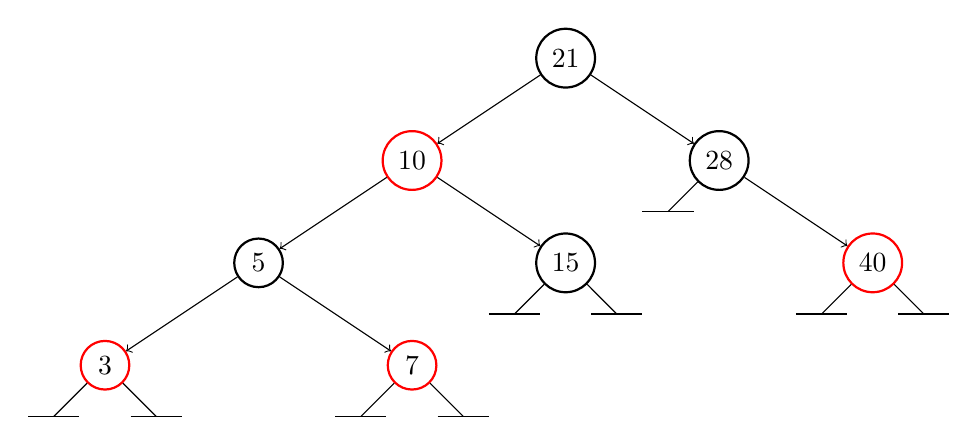
\begin{tikzpicture}[scale=0.65]
		\begin{scope}[every node/.style={circle,thick,draw}]
		\node 			(top) at (10, 10)   {$21$};
		
		\node[draw=red] (2-1) at (7,  8) 	{$10$};
		\node 			(2-2) at (13, 8) 	{$28$};
		
		\node 			(3-1) at (4,  6) 	{$5$};
		\node 			(3-2) at (10, 6) 	{$15$};
		\node[draw=red] (3-3) at (16, 6)    {$40$};
		
		\node[draw=red] (4-1) at (1,  4)	{$3$};
		\node[draw=red] (4-2) at (7,  4)	{$7$};
		\end{scope}
		
		
		\path [->] (top) edge (2-1);
		\path [->] (top) edge (2-2);
				
		\path [->] (2-1) edge (3-1);
		\path [->] (2-1) edge (3-2);
		\path [->] (2-2) edge (3-3);
		
		\path [->] (3-1) edge (4-1);
		\path [->] (3-1) edge (4-2);
		
		\path [-] (4-1) edge (0, 3);
		\draw (-0.5, 3) -- (0.5, 3);
		
		\path [-] (4-1) edge (2, 3);
		\draw (1.5, 3) -- (2.5, 3);
		
		\path [-] (4-2) edge (6, 3);
		\draw (5.5, 3) -- (6.5, 3);
		
		\path [-] (4-2) edge (8, 3);
		\draw (7.5, 3) -- (8.5, 3);
		
		\path [-] (3-2) edge (9, 5);
		\draw (8.5, 5) -- (9.5, 5);
		
		\path [-] (3-2) edge (11, 5);
		\draw (10.5, 5) -- (11.5, 5);
		
		\path [-] (2-2) edge (12, 7);
		\draw (11.5, 7) -- (12.5, 7);
		
		\path [-] (3-3) edge (15, 5);
		\draw (14.5, 5) -- (15.5, 5);
		
		\path [-] (3-3) edge (17, 5);
		\draw (16.5, 5) -- (17.5, 5);
		
		
		\end{tikzpicture}
	\end{center}
	\textit{Во всех следующих рисунках будет подразумеваться, что от каждой последней значащей ноды исходит соответствующее число фиктивных листьев.}
	
	
	\begin{preposition}
		Высота КЧД -- $O(\log n)$, где $n$ -- число ключей в дереве. Более точно: 
		\[
		h \leqslant 2\log_2(n+1)
		\]
	\end{preposition}
	\begin{proof}
		Так как нам интересна черная высота дерева, объединим красные и черные узлы с листов вверх по дереву. Получим следующее дерево:
		
		\TODO{Тут будет дерево}
		
		 \begin{center}
			\begin{tikzpicture}[scale=0.65]
			\begin{scope}[every node/.style={circle,thick,draw}]
			\node[ellipse]  	     (top) at (10, 10)   {$10/21$};
			
			\node[ellipse, draw=red] (2-1) at (6,  8) 	 {$3/5/10$};
			\node 			         (2-2) at (10, 8) 	 {$15$};
			\node[ellipse, draw=red] (2-3) at (14, 8)    {$28/40$};
			
			\end{scope}
			
			
			\path [->] (top) edge (2-1);
			\path [->] (top) edge (2-2);
			\path [->] (top) edge (2-3);
			
			
			\end{tikzpicture}
		\end{center}
	
	Такое дерево находится в классе 2-3-4-деревьев поиска (классификация по количеству возможных детей у узлов) с высотой $h' = black\_height(root)$. 
	
	Докажем, что в КЧ-дереве с $n$ ключами $n+1$ лист. База индукции верна: для дерева, в котором ровно один ключ, есть 2 листа. Осталось доказать переход. Пусть верно, что в дереве с $n-1$ ключом $n$ листьев. Возьмем два таких дерева, обозначим за $n_1$ и $n_2$. Тогда:
	\[
	leaves(t) = n_1 + 1 + n_2 + 1 = (n_1 + n_2 + 1) + 1 = nodes(t) + 1
	\]
	\end{proof}

	\subsection{Вставка и удаление}
	
	Так как КЧД является деревом поиска, для начала надо просто выполнить $tree\_insert$, чтобы вставить элемент в дерево. Но при этом может нарушиться несколько свойств дерева. Поэтому, нам необходимо поменять структуру. Делается это двумя операциями: \textit{перекрашивание} и \textit{поворот}. Если первая операция тривиальна, то вторая операция требует объяснения.
	
	\subsubsection{Поворот в КЧД}
	\textit{Правый поворот} -- это такая операция, которая выполняет следующее преобразование:
	\begin{center}
		\begin{tikzpicture}[scale=0.65]
		\begin{scope}[every node/.style={circle,thick,draw,minimum size=2em}]
		\node 			(topl) at (10, 10)   {$B$};
		
		\node 			(12-1) at (7,  8) 	{$A$};
		\node[ellipse] 	(12-2) at (13, 8) 	{$\gamma$};
		
		\node 			(13-1) at (4,  6) 	{$\alpha$};
		\node           (13-2) at (10,  6)   {$\beta$};
		
		
		\node 			(topr) at (22, 10)   {$A$};
		
		\node			(22-2) at (19,  8) 	{$\alpha$};
		\node 			(22-1) at (25,  8) 	{$B$};
		
		\node 			(23-1) at (22,  6) 	{$\beta$};
		\node           (23-2) at (28,  6)  {$\gamma$};
		\end{scope}
		
		\node (n) at (16, 8) {$\Rightarrow$};
		
		\path [->] (topl) edge (12-1);
		\path [->] (topl) edge (12-2);
		
		\path [->] (12-1) edge (13-1);
		\path [->] (12-1) edge (13-2);
		
		
		
		\path [->] (topr) edge (22-1);
		\path [->] (topr) edge (22-2);
		
		\path [->] (22-1) edge (23-1);
		\path [->] (22-1) edge (23-2);
		
		\end{tikzpicture}
	\end{center}
	
	\textit{Левый поворот} -- это обратная операция к правому повороту.
	
	После поворота инвариант дерева выполняется:
	\[
	\forall a \in \alpha \ \forall b \in \beta \ \forall c \in \gamma: \ a \leqslant A \leqslant b \leqslant B \leqslant c
	\]
	
	\subsection{Построение алгоритма}
	
	Теперь рассмотрим случаи, когда какую операцию необходимо выполнять. Нода, в которой написан $x$ -- та нода, которую мы вставили.
	\begin{enumerate}
		\item Первый случай требует от нас перекрасить наш граф:
		\begin{center}
			\begin{tikzpicture}[scale=0.65]
			\begin{scope}[every node/.style={circle,thick,draw,minimum size=2em}]
			\node 			(topl) at (10, 10)   {};
			
			\node[draw=red]	(12-1) at (7,  8) 	{};
			\node[draw=red]	(12-2) at (13, 8) 	{};
			
			\node[draw=red]	(13-1) at (4,  6) 	{$x$};
			
			
			\node[draw=red]	(topr) at (26, 10)   {$x$};
			
			\node			(22-1) at (23,  8) 	{};
			\node 			(22-2) at (29,  8) 	{};
			
			\node[draw=red]	(23-1) at (20,  6) 	{};
			\end{scope}
			
			\node (n) at (16, 8) {$\Rightarrow$};
			
			\path [->] (topl) edge (12-1);
			\path [->] (topl) edge (12-2);
			
			\path [->] (12-1) edge (13-1);
			
			
			
			\path [->] (topr) edge (22-1);
			\path [->] (topr) edge (22-2);
			
			\path [->] (22-1) edge (23-1);
			\end{tikzpicture}
		\end{center}
	
		\item Второй случай требует повернуть дерево:
		\begin{center}
			\begin{tikzpicture}[scale=0.65]
			\begin{scope}[every node/.style={circle,thick,draw,minimum size=2em}]
			\node 			(topl) at (10, 10)   {x};
			
			\node[draw=red]	(12-1) at (7,  8) 	{};
			\node[draw=red]	(12-2) at (13, 8) 	{};
			
			\node       	(13-1) at (10,  6) 	{$x$};
			
			
			\node[draw=red]	(topr) at (26, 10)   {$x$};
			
			\node			(22-1) at (23,  8) 	{};
			\node 			(22-2) at (29,  8) 	{};
			
			\node[draw=red]	(23-1) at (20,  6) 	{};
			\end{scope}
			
			\node (n) at (16, 8) {$\Rightarrow$};
			
			\path [->] (topl) edge (12-1);
			\path [->] (topl) edge (12-2);
			
			\path [->] (12-1) edge (13-1);
			
			
			
			\path [->] (topr) edge (22-1);
			\path [->] (topr) edge (22-2);
			
			\path [->] (22-1) edge (23-1);
			\end{tikzpicture}
		\end{center}
		
	\end{enumerate}
	
	
	
	
	
	
	
	
	
	
	
	
	
	
\end{document}